\documentclass[12pt, a4paper]{report}
\usepackage{graphicx}
\usepackage{amsmath}
\usepackage{float}
\usepackage{geometry}
\usepackage{fancyhdr}

% Configurações de Margens
\geometry{left=3cm,right=2cm,top=3cm,bottom=2cm}

% Cabeçalhos e rodapés
\pagestyle{fancy}
\fancyhf{}
\fancyhead[L]{Universidade Federal do Tocantins}
\fancyhead[R]{Análise Empírica de Algoritmos de Ordenação}
\fancyfoot[C]{\thepage}

% Início do Documento
\begin{document}

% Capa
\begin{titlepage}
    \centering
    
\includegraphics[width=0.3\textwidth]{uft_logo.png}\\[1cm]
    \vspace{1cm}
    \textbf{\Large UNIVERSIDADE FEDERAL DO TOCANTINS}\\[0.5cm]
    \textbf{\large CURSO DE GRADUAÇÃO EM CIÊNCIA DA COMPUTAÇÃO}\\[2cm]
    
    \textbf{\large Ester Arraiz de Matos\\Victor Emanuel da Silva Campelo\\Laurinda Nhanga Mona}\\[2cm]
    
    \textbf{\LARGE ANÁLISE EMPÍRICA DE ALGORITMOS DE ORDENAÇÃO}\\[7cm]
    
    Palmas, TO\\
    2024
    
\end{titlepage}

% Resumo
\chapter*{Resumo}
Este trabalho analisa e compara o desempenho de seis algoritmos de ordenação: Bubble Sort, Selection Sort, Insertion Sort, Merge Sort, Quick Sort e Heap Sort. A pesquisa visa realizar uma análise empírica baseada em testes com diferentes tamanhos de listas (1.000, 10.000, 50.000 e 100.000 elementos) e distribuições (ordenadas, inversamente ordenadas e aleatórias). Foram avaliadas as métricas de tempo de execução, número de comparações e trocas realizadas. Os resultados mostram que Heap Sort e Merge Sort foram os mais eficientes para listas grandes, enquanto Bubble Sort, Selection Sort e Insertion Sort tiveram desempenho insatisfatório.

\vspace{0.5cm}

\textbf{Palavras-chave:} Algoritmos de Ordenação. Análise Empírica. Tempo de Execução.

% Abstract
\chapter*{Abstract}
This work analyzes and compares the performance of six sorting algorithms: Bubble Sort, Selection Sort, Insertion Sort, Merge Sort, Quick Sort, and Heap Sort. The research aims to conduct an empirical analysis based on tests with different list sizes (1,000, 10,000, 50,000, and 100,000 elements) and distributions (sorted, inversely sorted, and random). The metrics evaluated were execution time, number of comparisons, and swaps. The results show that Heap Sort and Merge Sort were the most efficient for large lists, while Bubble Sort, Selection Sort, and Insertion Sort showed unsatisfactory performance.

\vspace{0.5cm}

\textbf{Keywords:} Sorting Algorithms. Empirical Analysis. Execution Time.

% Introdução
\chapter{Introdução}
A ordenação de dados é uma operação crucial na ciência da computação, utilizada em
uma ampla gama de aplicações, desde a organização de grandes volumes de informações até a
execução de algoritmos mais complexos. Os métodos de ordenação são a base para o
desempenho eficiente de muitos sistemas, que precisam ser rápidos e eficazes ao lidar com
cargas de trabalho críticas. Portanto, a escolha do melhor algoritmo de ordenação influencia
significativamente o desempenho geral de um sistema.
Cada algoritmo de ordenação possui características únicas em termos de eficiência e
desempenho. Alguns são mais adequados para listas pequenas e simples, enquanto outros são
projetados para processar grandes volumes de dados de maneira mais eficaz. Além disso, a
própria disposição dos dados, como já ordenados, não ordenados, invertidos ou aleatórios,
impacta significativamente o desempenho dos algoritmos.
Assim, esta pesquisa tem como objetivo realizar uma análise empírica com base nos
testes de seis algoritmos de ordenação amplamente conhecidos: Bubble Sort, Selection Sort,
Insertion Sort, Merge Sort, Quick Sort e Heap Sort. O trabalho busca oferecer uma base
teórica sobre todos os algoritmos, mas também apresentar resultados de testes e comparações
com diferentes cargas, tamanhos de dados de entrada de 1.000, 10.000, 50.000 e 100.000,
com esses elementos ordenados, inversamente ordenados e aleatórios.
Dessa forma, três fatores principais serão analisados durante os testes: tempo de
execução, quantidade de comparações e quantidade de trocas realizadas pelo algoritmo.
Essas métricas ajudarão na comparação das vantagens e desvantagens de cada método em
diferentes circunstâncias e tamanhos de dados.

% Revisão Teórica
\chapter{Revisão Teórica}
\section{Bubble Sort}
O Bubble Sort é um dos algoritmos de ordenação mais simples, muitas vezes
ensinado como uma introdução ao tema. Ele funciona comparando pares de elementos
adjacentes e trocando-os caso estejam na ordem errada. A complexidade de tempo desse
algoritmo é O(n²), o que significa que, em listas grandes, ele pode se tornar bastante lento. No
entanto, no melhor caso, quando a lista já está ordenada, ele pode operar em O(n). O
interessante é que ele é um algoritmo in-place, ou seja, ordena os elementos diretamente na
lista original sem exigir memória extra significativa. Além disso, é um algoritmo estável, pois
não altera a ordem de elementos iguais, garantindo que eles permaneçam na mesma posição
relativa.

\section{Selection Sort}
O Selection Sort é um pouco mais eficiente que o Bubble Sort, mas ainda assim não é
o ideal para listas grandes. Ele funciona selecionando repetidamente o menor (ou maior)
elemento da parte não ordenada e movendo-o para o início da lista. A complexidade do
Selection Sort é também O(n²), independentemente do estado da lista, o que pode torná-lo
ineficiente em muitos casos. Assim como o Bubble Sort, é um algoritmo in-place, não
utilizando memória extra significativa. No entanto, ele não é estável, o que significa que a
ordem de elementos iguais pode ser alterada durante as trocas.

\section{Insertion Sort}
O Insertion Sort se destaca entre os algoritmos de ordenação por sua simplicidade e
eficiência em listas pequenas ou quase ordenadas. Ele funciona construindo uma sublista
ordenada à medida que percorre a lista original, inserindo elementos na posição correta. Sua
complexidade de tempo é O(n²) no pior e no caso médio, mas pode ser O(n) quando a lista já
está ordenada. É um algoritmo in-place, o que significa que ordena na própria lista sem exigir
espaço extra. Além disso, é estável, pois preserva a ordem relativa dos elementos iguais,
tornando-o uma escolha adequada em muitos casos.

\section{Merge Sort}
O Merge Sort é um algoritmo eficiente e amplamente utilizado, especialmente em
situações que exigem ordenação de grandes volumes de dados. Ele adota uma abordagem de
divisão e conquista, dividindo repetidamente a lista em sublistas menores, até que cada
sublista contenha apenas um elemento, e então mescla essas sublistas de volta em uma lista
ordenada. Com uma complexidade de tempo de O($n \log n$) em todos os casos, o Merge Sort é
bastante eficiente. No entanto, ele não é um algoritmo in-place, pois requer memória
adicional para armazenar as sublistas durante o processo. Por outro lado, é um algoritmo
estável, o que significa que mantém a ordem dos elementos iguais.


\section{Quick Sort}
O Quick Sort é conhecido por sua eficiência em uma variedade de cenários,
especialmente em listas grandes. Ele também utiliza a estratégia de divisão e conquista,
escolhendo um "pivô" e particionando a lista em elementos menores e maiores do que esse
pivô. Sua complexidade de tempo média é O($n \log n$), mas no pior caso, pode chegar a O(n²),
especialmente se o pivô escolhido não for bem equilibrado. O Quick Sort é in-place, pois
ordena diretamente na lista original, embora possa usar memória adicional para as chamadas
recursivas. No entanto, ele não é estável, podendo alterar a ordem relativa de elementos
iguais.

\section{Heap Sort}
O Heap Sort é um algoritmo eficiente que utiliza uma estrutura de dados chamada
heap para realizar a ordenação. Ele constrói um heap a partir da lista e, em seguida, extrai
repetidamente o maior elemento (ou o menor, dependendo da ordem desejada) para construir
a lista ordenada. Com uma complexidade de tempo de O($n \log n$) em todos os casos, o Heap
Sort é bastante eficiente e ideal para grandes volumes de dados. Além disso, ele é in-place,
pois utiliza a própria lista para realizar a ordenação. No entanto, assim como o Quick Sort,
não é estável, o que pode afetar a ordem relativa de elementos iguais.
Essa revisão fornece uma visão geral das características teóricas de cada algoritmo,
preparando o terreno para a análise prática que será realizada posteriormente. Compreender
esses aspectos é fundamental para saber qual algoritmo utilizar em diferentes situações e
como eles se comportam sob várias condições.

% Metodologia
\chapter{Metodologia}
\section{Ambiente de Testes}
Os testes foram realizados em um computador Lenovo Ideapad 3i com processador Intel i5, 8 GB de RAM, SSD de 256 GB, executando o sistema operacional Windows 11 Pro. O ambiente de desenvolvimento utilizado foi Python 3.12, no Visual Studio Code.

\section{Implementação dos Algoritmos}
Neste trabalho, foram implementados seis algoritmos de ordenação: Bubble Sort,
Selection Sort, Insertion Sort, Merge Sort, Quick Sort e Heap Sort. Cada algoritmo foi
desenvolvido de forma independente para medir o número de comparações e trocas
realizadas, além do tempo de execução para listas com diferentes tamanhos e distribuições.
\subsection*{Descrição dos Algoritmos:}

\begin{enumerate}
    \item \textbf{Bubble Sort:}
    \begin{itemize}
        \item A cada iteração, o algoritmo compara dois elementos adjacentes e os troca de lugar se estiverem fora de ordem. O processo é repetido até que a lista esteja completamente ordenada.
        \item \textbf{Complexidade de Tempo:} O($n^2$)
    \end{itemize}

    \item \textbf{Selection Sort:}
    \begin{itemize}
        \item O algoritmo encontra o menor elemento da lista e o move para a primeira posição. Em seguida, repete o processo para o restante da lista até que ela esteja ordenada.
        \item \textbf{Complexidade de Tempo:} O($n^2$)
    \end{itemize}

    \item \textbf{Insertion Sort:}
    \begin{itemize}
        \item O algoritmo percorre a lista, inserindo cada elemento em sua posição correta, movendo os elementos maiores para a direita conforme necessário.
        \item \textbf{Complexidade de Tempo:} O($n^2$)
    \end{itemize}

    \item \textbf{Merge Sort:}
    \begin{itemize}
        \item O algoritmo divide recursivamente a lista ao meio, ordena cada uma das metades e as combina (merge) para formar uma lista ordenada final.
        \item \textbf{Complexidade de Tempo:} O($n \log n$)
    \end{itemize}

    \item \textbf{Quick Sort:}
    \begin{itemize}
        \item O algoritmo seleciona um pivô, particiona a lista em dois grupos (menores e maiores que o pivô), e ordena recursivamente cada parte.
        \item \textbf{Complexidade de Tempo:} O($n \log n$) em média, e O($n^2$) no pior caso, dependendo da escolha do pivô.
    \end{itemize}

    \item \textbf{Heap Sort:}
    \begin{itemize}
        \item O algoritmo constrói uma árvore binária do tipo heap e remove o maior elemento (raiz) repetidamente até que a lista esteja ordenada.
        \item \textbf{Complexidade de Tempo:} O($n \log n$)
    \end{itemize}
    
    
\end{enumerate}
Todos os algoritmos foram implementados em Python utilizando uma classe chamada SortMetrics, que foi usada para armazenar o número de comparações e trocas realizadas durante a execução de cada algoritmo.

\section{Procedimento para Medir Desempenho}
O desempenho de cada algoritmo foi avaliado com base em três métricas principais:
\begin{itemize}
    \item \textbf{Tempo de execução:} Medido em milissegundos.
    \item \textbf{Número de comparações:} Quantidade de vezes que os elementos foram comparados durante a execução.
    \item \textbf{Número de trocas:} Quantidade de vezes que dois elementos trocaram de posição.
\end{itemize}

\subsection*{Procedimento para Medição}

\textbf{Geração dos Arrays de Teste:} Foram gerados três tipos de listas de diferentes tamanhos (1.000, 10.000, 50.000, 100.000 elementos):
\begin{itemize}
    \item \textbf{Listas Ordenadas:} Elementos em ordem crescente.
    \item \textbf{Listas Inversamente Ordenadas:} Elementos em ordem decrescente.
    \item \textbf{Listas Aleatórias:} Elementos dispostos aleatoriamente.
\end{itemize}
A geração das listas foi feita através da função \texttt{generate\_test\_arrays}, que assegura que as listas sejam criadas de acordo com as características desejadas para os testes.

\textbf{Medição do Tempo de Execução:} O tempo de execução foi medido utilizando as funções \texttt{time.time()} e \texttt{time.perf\_counter()}, sendo esta última utilizada para maior precisão em medições curtas. O tempo foi registrado no início e no final de cada execução de algoritmo, e a diferença foi calculada para obter o tempo total em milissegundos.

\textbf{Execução dos Testes:} Para cada algoritmo, os testes foram repetidos em diferentes distribuições de listas (ordenadas, inversamente ordenadas e aleatórias) e em vários tamanhos de lista (1.000, 10.000, 50.000, 100.000 elementos). Esse procedimento permitiu uma análise detalhada do desempenho de cada algoritmo sob diversas condições, resultando em uma avaliação completa de eficiência em termos de tempo de execução, comparações e trocas.

% Resultados
\chapter{Resultados}
\section{Listas Aleatórias}
Os resultados para listas aleatórias mostraram que Merge Sort e Heap Sort tiveram tempos de execução mais rápidos, enquanto Bubble Sort foi o mais lento.

\begin{figure}[H]
    \centering
    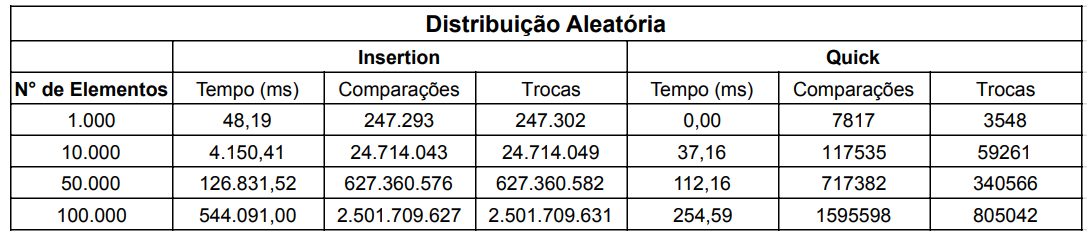
\includegraphics[width=0.9\textwidth]{listas/aleatorio1.png}
    \caption{Distribuição Aleatória (Insertion e Quick)}
    \label{fig:aleatorio1}
\end{figure}
\begin{figure}[H]
    \centering
    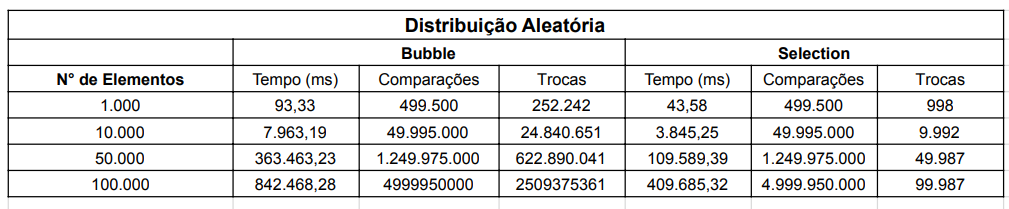
\includegraphics[width=0.9\textwidth]{listas/aleatorio2.png}
    \caption{Distribuição Aleatória (Bubble e Selection)}
    \label{fig:aleatorio2}
\end{figure}
\begin{figure}[H]
    \centering
    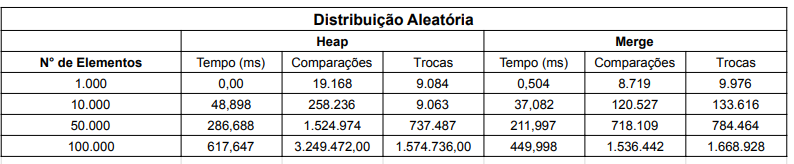
\includegraphics[width=0.9\textwidth]{listas/aleatorio3.png}
    \caption{Distribuição Aleatória (Heap e Merge)}
    \label{fig:aleatorio3}
\end{figure}

\section{Listas Ordenadas}
Nos testes com listas ordenadas, Quick Sort apresentou pior desempenho devido à escolha do pivô, enquanto Merge Sort se destacou.
\begin{figure}[H]
    \centering
    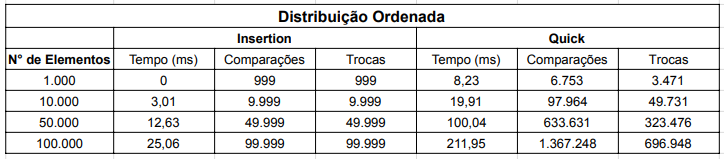
\includegraphics[width=0.9\textwidth]{listas/ordenada1.png}
    \caption{Distribuição Ordenada (Insertion e Quick)}
    \label{fig:ordenada1}
\end{figure}
\begin{figure}[H]
    \centering
    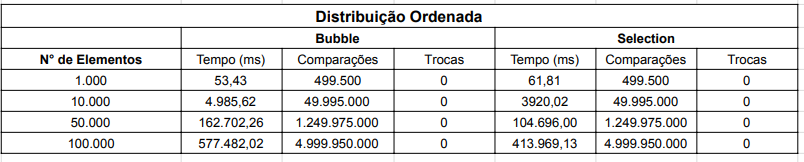
\includegraphics[width=0.9\textwidth]{listas/ordenada2.png}
    \caption{Distribuição Ordenada (Bubble e Selection)}
    \label{fig:ordenada2}
\end{figure}
\begin{figure}[H]
    \centering
    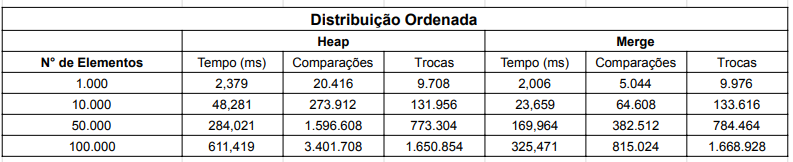
\includegraphics[width=0.9\textwidth]{listas/ordenada3.png}
    \caption{Distribuição Ordenada (Heap e Merge)}
    \label{fig:ordenada3}
\end{figure}

\section{Listas Inversamente Ordenadas}
Em listas inversamente ordenadas, Insertion Sort teve o pior desempenho, confirmando sua ineficiência em dados muito desorganizados.

\begin{figure}[H]
    \centering
    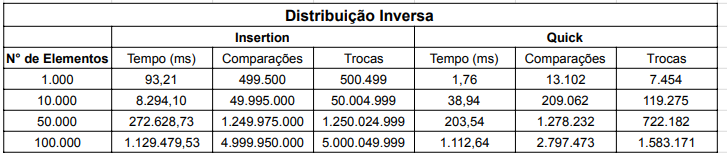
\includegraphics[width=0.9\textwidth]{listas/inversa1.png}
    \caption{Distribuição Inversa (Insertion e Quick)}
    \label{fig:inversa1}
\end{figure}
\begin{figure}[H]
    \centering
    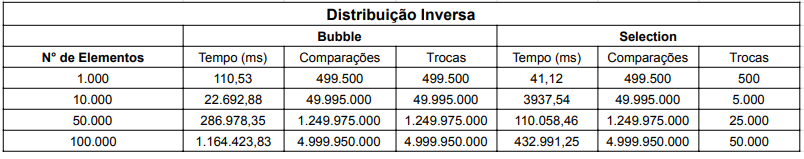
\includegraphics[width=0.9\textwidth]{listas/inversa2.png}
    \caption{Distribuição Inversa (Bubble e Selection}
    \label{fig:inversa2}
\end{figure}
\begin{figure}[H]
    \centering
    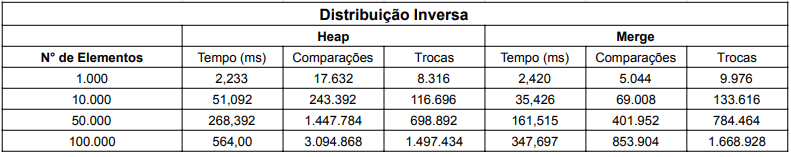
\includegraphics[width=0.9\textwidth]{listas/inversa3.png}
    \caption{Distribuição Inversa (Heap e Merge)}
    \label{fig:inversa3}
\end{figure}


% Discussão
\chapter{Discussão}
Os resultados dos algoritmos de ordenação em diferentes tamanhos de listas e distribuições de dados estão alinhados com as expectativas teóricas, em grande parte, confirmando o comportamento previsto pela análise de complexidade.

\begin{enumerate}
    \item \textbf{Heap Sort e Merge Sort}
    \begin{itemize}
        \item Heap Sort e Merge Sort apresentaram tempos de execução consistentes com sua complexidade $O(n \log n)$, destacando-se em listas maiores, onde a eficiência de ambos foi visível. Por exemplo, em uma lista aleatória de 100.000 elementos, o Heap Sort levou cerca de 617 ms, enquanto o Merge Sort foi ligeiramente mais rápido, com 449 ms, o que reflete bem as expectativas para esse tipo de complexidade.
    \end{itemize}

    \item \textbf{Quick Sort}
    \begin{itemize}
        \item Quick Sort também mostrou bom desempenho, especialmente em listas aleatórias, porém teve desempenho inferior ao Merge Sort em listas ordenadas, como esperado, devido ao aumento do número de comparações em cenários desfavoráveis. Isso ocorre porque o pivô escolhido impacta diretamente a eficiência.
    \end{itemize}
    
    \item \textbf{Insertion Sort, Bubble Sort e Selection Sort}
    \begin{itemize}
        \item Com sua complexidade $O(n^2)$, Insertion Sort, Bubble Sort e Selection Sort apresentaram desempenhos bem mais lentos em listas grandes, como previsto. Para listas inversamente ordenadas, o Insertion Sort apresentou tempos extremamente altos (ex.: 1.129.479 ms para 100.000 elementos), devido ao grande número de comparações e trocas necessárias.
    \end{itemize}
    
\end{enumerate}
\section{Considerações sobre a Facilidade de Implementação, Uso de Memória e Estabilidade}

\subsection{Facilidade de Implementação}
\begin{itemize}
    \item Bubble Sort, Selection Sort e Insertion Sort são relativamente simples de implementar devido à sua lógica direta, mas essa simplicidade vem acompanhada de um custo de desempenho elevado em listas grandes.
    \item Heap Sort e Quick Sort exigem uma implementação mais elaborada, especialmente no particionamento (Quick) e na heapificação (Heap). No entanto, essas complexidades são compensadas pelo melhor desempenho.
    \item Merge Sort é fácil de implementar recursivamente, mas a necessidade de espaço adicional torna sua otimização um pouco mais desafiadora.
\end{itemize}

\subsection{Uso de Memória}
\begin{itemize}
    \item Merge Sort exige espaço adicional proporcional ao tamanho da lista para armazenar os subarrays temporários, o que pode ser um fator limitante em sistemas com memória restrita.
    \item Heap Sort e Quick Sort são algoritmos "in-place", ou seja, não precisam de espaço extra significativo além da lista original, sendo mais eficientes em termos de uso de memória.
    \item Bubble Sort, Selection Sort e Insertion Sort também são algoritmos "in-place", mas o uso de tempo excessivo obscurece sua vantagem em relação à memória.
\end{itemize}

\subsection{Estabilidade}
\begin{itemize}
    \item Merge Sort é um algoritmo estável, mantendo a ordem relativa dos elementos iguais, o que é uma característica importante em determinadas aplicações.
    \item Quick Sort e Heap Sort não são estáveis, ou seja, a ordem dos elementos iguais pode ser alterada durante a ordenação.
    \item Bubble Sort e Insertion Sort são estáveis, o que pode ser um ponto positivo quando a estabilidade é uma exigência, apesar de sua ineficiência com grandes conjuntos de dados.
\end{itemize}

\section{Discussão sobre as Limitações do Trabalho e Sugestões para Estudos Futuros}

\subsection{Limitações do Trabalho}
\begin{itemize}
    \item O experimento foi limitado a alguns tamanhos de listas. Ampliar o intervalo de tamanhos testados ajudaria a entender melhor como os algoritmos se comportam em diferentes escalas.
    \item A implementação do Quick Sort não usou a mediana de três como pivô, uma técnica que poderia ter melhorado seu desempenho em listas ordenadas e inversamente ordenadas.
    \item O uso de memória não foi diretamente medido. Analisar esse aspecto mais detalhadamente seria útil para avaliar o impacto dos algoritmos em sistemas com restrições de memória.
\end{itemize}

\subsection{Sugestões para Estudos Futuros}
\begin{itemize}
    \item \textbf{Otimização do pivô no Quick Sort:} Implementar o Quick Sort utilizando a mediana de três ou outras estratégias de seleção de pivô para melhorar o desempenho em listas quase ordenadas ou ordenadas inversamente.
    \item \textbf{Testes com distribuições adicionais:} Além das distribuições de listas ordenadas, inversamente ordenadas e aleatórias, testar os algoritmos com listas quase ordenadas ou com muitos valores repetidos poderia fornecer insights adicionais.
    \item \textbf{Análise de uso de memória:} Realizar uma análise mais aprofundada do uso de memória de cada algoritmo, especialmente para grandes listas, ajudaria a entender melhor os trade-offs entre tempo de execução e espaço consumido.
    \item \textbf{Exploração de paralelismo:} Explorar versões paralelas dos algoritmos, especialmente Merge Sort e Quick Sort, pode ser interessante para avaliar o desempenho em sistemas multicore, onde o paralelismo pode reduzir significativamente os tempos de execução em listas grandes.
\end{itemize}

Esses pontos abririam novas oportunidades para otimizações e análises, fornecendo uma visão mais completa do desempenho e da aplicabilidade dos algoritmos de ordenação em diferentes contextos.


\chapter{Conclusão}
Neste trabalho, analisamos e comparamos o desempenho de seis algoritmos de ordenação: Bubble Sort, Selection Sort, Insertion Sort, Merge Sort, Quick Sort e Heap Sort. Os resultados obtidos confirmaram as expectativas teóricas sobre a complexidade de cada um, revelando que Heap Sort e Merge Sort se destacam pela eficiência em listas grandes. Por outro lado, os algoritmos Insertion Sort, Bubble Sort e Selection Sort mostraram-se inadequados para grandes volumes de dados, confirmando sua ineficiência.
Além disso, a análise ressaltou a relação entre a facilidade de implementação, o uso de memória e a estabilidade dos algoritmos. Embora os algoritmos mais simples sejam fáceis de implementar, seu desempenho pode ser insatisfatório em aplicações práticas, o que é um ponto importante a ser considerado.
Identificamos também algumas limitações no estudo, como a necessidade de testar uma variedade maior de tamanhos de listas e a falta de uma análise mais detalhada sobre o uso de memória. Para futuras pesquisas, sugerimos explorar otimizações no Quick Sort, avaliar distribuições de dados específicas e considerar implementações paralelas dos algoritmos.
Em suma, este trabalho destaca a importância de compreender as características e o desempenho dos algoritmos de ordenação, oferecendo insights valiosos para escolhas informadas no desenvolvimento de software e em aplicações práticas.


% Referências
\chapter*{Referências}
\addcontentsline{toc}{chapter}{Referências}

PEDROSO, Alexandre da Silva; CINTRA, Fausto Gonçalves. Estudo analítico do desempenho de algoritmos de ordenação. Revista EduFatec, 2022.

SOUZA, Jackson É. G.; RICARTE, João V. G. Algoritmos de ordenação: um estudo comparativo. Universidade Federal Rural do Semi-Árido, 2024.

SAMPAIO NETO, Nelson Cruz. Análise de algoritmos: algoritmos de ordenação. Universidade Federal do Pará, 2024.

BIGONHA, Roberto S. Complexidade de algoritmos. Universidade Federal de Minas Gerais, 2006.

\end{document}



